

% This is based on the LLNCS.DEM the demonstration file of
% the LaTeX macro package from Springer-Verlag
% for Lecture Notes in Computer Science,
% version 2.4 for LaTeX2e as of 16. April 2010
%
% See http://www.springer.com/computer/lncs/lncs+authors?SGWID=0-40209-0-0-0
% for the full guidelines.
%
\documentclass{llncs}
\usepackage{lipsum}
\usepackage{graphicx}
\usepackage[export]{adjustbox}
\usepackage{float}
\usepackage{hyperref}

\begin{document}
\title{Summary, Application Example and Critique of the Paper: Predictive Process Monitoring Methods - Which one Suits Me Best?}
\author{Fabian Braun}
\institute{Ludwig-Maximilians-Universit\"at M\"unchen}

\maketitle 
\begin{center}
Masterseminar ``Recent Developments in Data Science - Process Mining'' \\
Wintersemester 2018/19
\end{center}

\begin{abstract}
The abstract should summarize the contents of the paper
using at least 70 and at most 150 words. It will be set in 9-point
font size and be inset 1.0 cm from the right and left margins.
There will be two blank lines before and after the Abstract. \dots
\keywords{Keyword1, Keyword2, ...}
\end{abstract}

\section{Introduction}
Compliance monitoring in businesses, the assessment whether the execution of intern processes is on par with policies, 
regulations and laws, is generally bound to a reactive approach. Violations are only identified after their occurrence, 
without the possibility of preventing them in the first place \cite{di2018predictive}.
In Contrast to these reactive approaches, predictive process monitoring methods allow the user to continuously monitor 
currently ongoing processes. These Predictive approaches provide predictions about an expected outcome, based on the 
current state and the preliminary information of a process.
With a large amount of literature describing these techniques becoming available, the paper by Di Francescomarino, Ghidini, 
Maggi and Milani aims to order and classify the different approaches currently developing in the field, by developing 
a value-driven framework to help researchers identifying upcoming challenges and companies finding suitable 
approaches for their requirements.
\paragraph{}
In this review, first a brief summary of the paper {\textit{"Predictive Monitoring Methods - Which one Suits Me Best?"} is given. 
In Section \ref{sec:app} the specified concepts are then further explained by an application example. At last Section \ref{sec:crit} comprises 
a critique of the work, depicting three strong and weak points of the paper.


\section{Summary}\label{sec:sum}
The papers main goal is the implementation of a framework that allows researches to get a quick overview of and identify upcoming challenges 
in the field of predictive process monitoring. To develop such a framework, a systematic literature review was carried out to identify 
the current state of the art in the field. This process was divided into two separate phases. In the first step the review protocol was defined, 
by formulating the underlying research question, identifying the collections of papers to be analysed, defining the inclusion and exclusion criteria and 
formulating the data extraction strategy \cite{di2018predictive}.
\paragraph{}
In the second phase the final list of papers was produced by applying the protocol setup in the first phase.
By applying a keyword based search on electronic libraries, including terms such as {\textit{"predictive", "business process"} or {\textit{"process mining"}, a primary collection of 780 papers was identified.
These papers where then reviewed considering  the inclusion and exclusion criteria, resulting 55 works chosen to be analysed and categorised, according to the underlying 
research question: {\textit{"How can the body of relevant academic publications within the field of predictive process monitoring be classified as a framework?"}.
By further refining this research question, four main categories for the distinction of the approaches were defined \cite{di2018predictive}:
\begin{itemize}
    \item[$\bullet$] "What aspects of the process are predicted?"
    \item[$\bullet$] "What input is required?"
    \item[$\bullet$] "What families of algorithms are used?"
    \item[$\bullet$] "What existing tools support the approach?"
\end{itemize}

The final 55 papers where then further analysed, by firstly extracting standard meta-data, like the author or year of publication.
After that, according to the four main categories deducted from the research question, for each work the type of prediction, the required data, the family of 
algorithms used and tools that support the approach were extracted. Furthermore domains for which the approaches are applicable, such as {\textit{"automotive"} 
or {\textit{"financial"} were determined and used as an additional attribute. The prediction type was emphasised as the main dimension to classify predictive 
process monitoring techniques and further subdivided into three categories of prediction types \cite{di2018predictive}.

\subsubsection{Numeric Predictions} are grouped into time and cost predictions. Time predictions are a versatile group, consisting of approaches that report 
information about elapsed, sojourn and remaining time for each state within the transition system. The collected information is applied to make predictions 
about the completion time of a process. Cost predictions on the other hand leverage a process model extended with costs, considering information about production, volume and time \cite{di2018predictive}.

\subsubsection{Categorial Predictions} are further split into risk and outcome predictions. Former are outcome-oriented, including approaches that minimize process risks by 
applying process models. These approaches utilise decision trees generated from the logs of past executions, which are then processed, resulting in 
probabilities returned to the user. The other group are categorial outcome predictions, which consider the fulfilment of predicates. In contrast to outcome predictions, 
most approaches evaluated in the paper of NAME, NAME und NAME do not apply any explicit model. Instead, frameworks that leverage the sequence of events and data payload 
of the last activity are applied to make predictions \cite{di2018predictive}.

\subsubsection{Next Activities Predictions} try to predict a sequence of future activities and their corresponding data payloads, by studying the previously observed activities \cite{di2018predictive}.

\vspace{10 mm}

The results of the paper are condensed into the tables \ref{fig:tab1} and \ref{fig:tab2}. Read from left to right, the tables distinguish approaches utilizing the four criteria 
deduced from the literature review, guiding readers to one of the 55 reviewed approaches.

\begin{table}[H]
    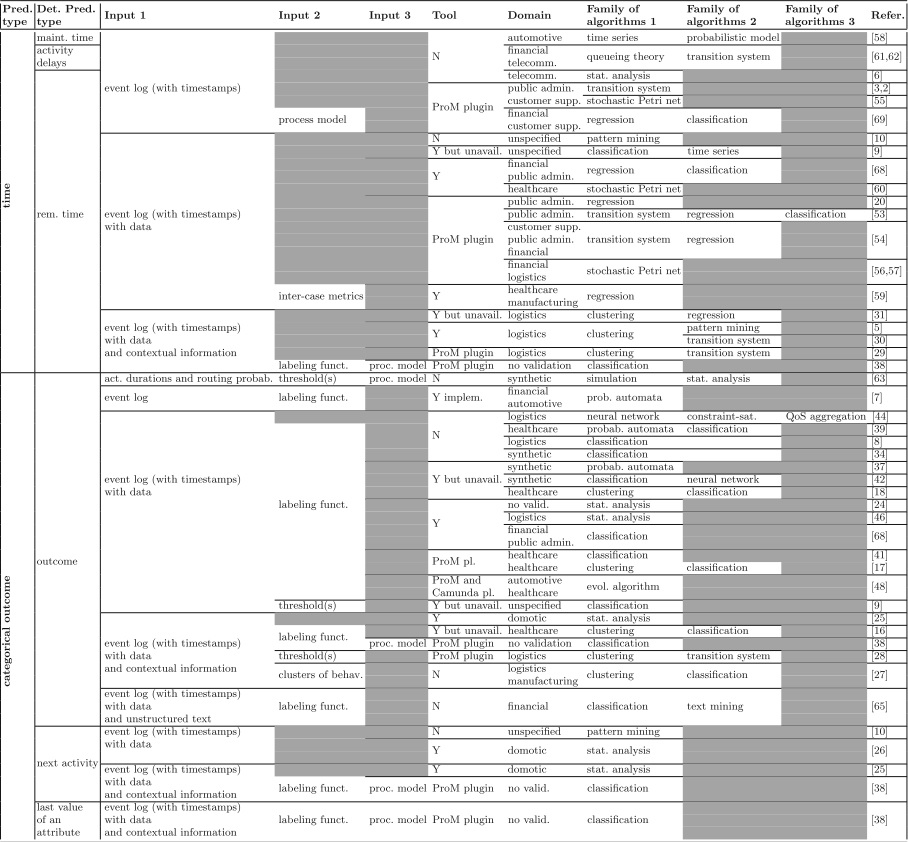
\includegraphics[width=1\linewidth,center]{tabelle1.jpg}
    \caption{Predictive process monitoring framework: time and categorical outcome predictions \cite{di2018predictive}}
    \label{fig:tab1}
\end{table}

\begin{table}[H]
    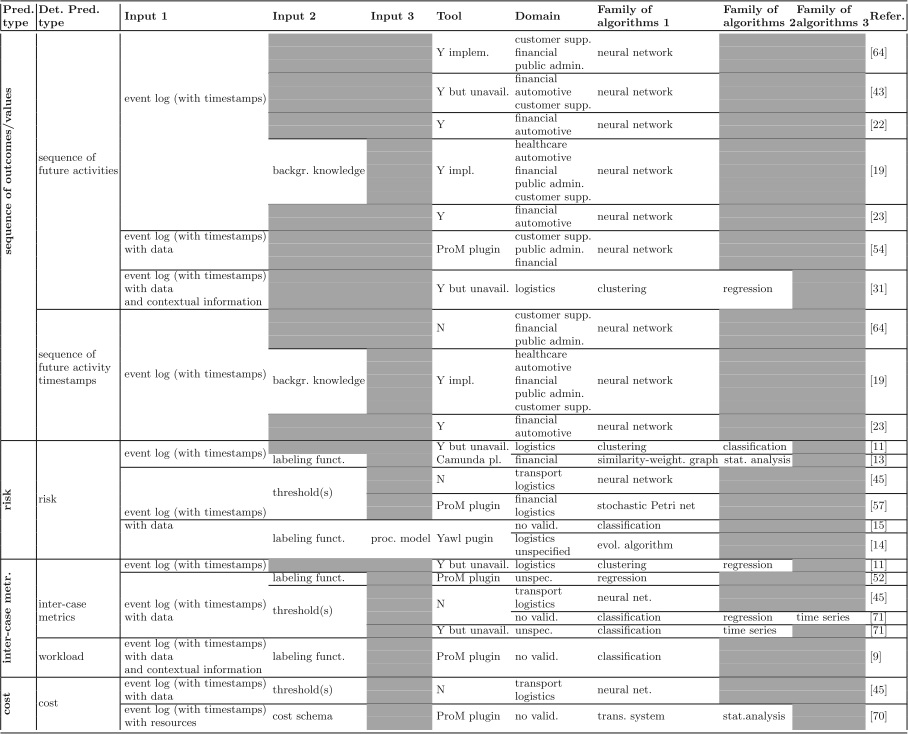
\includegraphics[width=1\linewidth,center]{tabelle2.jpg}
    \caption{Predictive process monitoring framework: sequence of outcomes/values, risk, inter-case metrics, cost \cite{di2018predictive}}
    \label{fig:tab2}
\end{table}

\section{Application Example}\label{sec:app}
In this passage the resulting tables \ref{fig:tab1} and \ref{fig:tab2} are applied to the simple example of a three step production line for self aware robots.
In activity A, body and limbs are assembled. This step is dependent on the availability of parts. Furthermore an event log containing assembly and waiting times is laid out.
Activity B is the quality assurance step for consciousness-independent functions. Basic motor functions are tested. The testing is dependent on the previous assembly of robot bodies. 
An event log containing testing and waiting times is laid out.
In the last Activity C, the artificial consciousness is simply uploaded to the robot body. Due to the software architecture and capacity of the factory the upload can only be implemented 
in parallel for ten soon to be self aware robots at a time.
The factory operators have noticed great fluctuations in the time it takes to fill up the ten spots for the consciousness upload in activity C, descending from delays in 
assembly or product testing. They decide to apply predictive process monitoring to proactively identify and counteract delays. To find a suitable approach they apply their problem to the 
tables \ref{fig:tab1} and \ref{fig:tab2}.
\paragraph{}
Going through the table from left to right, first the prediction type has to be determined. In the case of the self aware robot factory, it is time, more precisely activity delays.
The second category are the available inputs. For this example, there are time stamped event logs and a process model describing the connection between activities A, B and C available.
The third relevant category for the operators is the domain for which the approaches are most suitable. In this case, manufacturing.
Lastly the family of applied algorithms is considered, since the developers of the company already have experience with regression and stochastic Petri nets.
Considering the prediction and input type, as well as the family of algorithms the companies' developers are familiar with, the papers \cite{rogge2015time} and \cite{verenich2017white}, 
are chosen to be further reviewed.
Since the paper \cite{senderovich2017intra} is more suitable for the manufacturing domain and also applies regression, the operators decide to also consider it, even though it would require 
additional input, in the form of inter-case metrics, to be generated.






\section{Strong and Weak Points}\label{sec:crit}

\subsection{Strong Points}
well formulation what the paper tries to achieve
--> formulation of a research question and splitting it top down into smaller points of interest --> well structured
Convincing modus operandi for the selection and review of the subject.
Overseeable presentation of results in the form of tables. Easily implementable for businesses to find fitting approaches.

\subsection{Weak Points}
Some passages are though to read, because the sentences get very long
A lot of repetition. review process is described in some detail within the introduction and then again within a separate section



\bibliographystyle{acm}
\bibliography{literature}


\end{document}

              
 
